\documentclass[11pt,a4paper]{article}

% --- Packages ---
\usepackage[utf8]{inputenc}
\usepackage[T1]{fontenc}
\usepackage[margin=2.5cm]{geometry}
\usepackage{graphicx}
\usepackage{booktabs}
\usepackage{hyperref}
\usepackage{amsmath}
\usepackage{fancyhdr}
\usepackage{titlesec}
\usepackage{caption}
\usepackage{float}
\usepackage{parskip}
\graphicspath{{figures/}}

% --- Header / Footer ---
\pagestyle{fancy}
\fancyhf{}
\fancyhead[L]{\small Intro to Machine Learning Group Project}
\fancyhead[R]{\small Dublin Air Quality Forecasting}
\fancyfoot[C]{\thepage}
\renewcommand{\headrulewidth}{0.4pt}

% --- Section formatting ---
\titleformat{\section}{\large\bfseries}{\thesection.}{0.5em}{}
\titleformat{\subsection}[runin]{\normalsize\bfseries}{\thesubsection}{0.5em}{}[. \hspace{0.5em}]
\titlespacing{\subsection}{0pt}{1em}{0pt}

% --- Hyperref setup ---
\hypersetup{
	colorlinks=true,
	linkcolor=black,
	urlcolor=blue,
	citecolor=black
}

\begin{document}
	
	% ============================================================
	% TITLE PAGE
	% ============================================================
	\begin{titlepage}
		\centering
		\vspace*{2cm}
		
		{\Huge\bfseries Forecasting Next-Day PM2.5 in\\[6pt]
			Dublin Using Mobile Air Quality,\\[6pt]
			Weather, and Traffic Data\par}
		
		\vspace{1cm}
		{\Large Intro to Machine Learning Group Project\par}
		
		\vspace{2cm}
		
		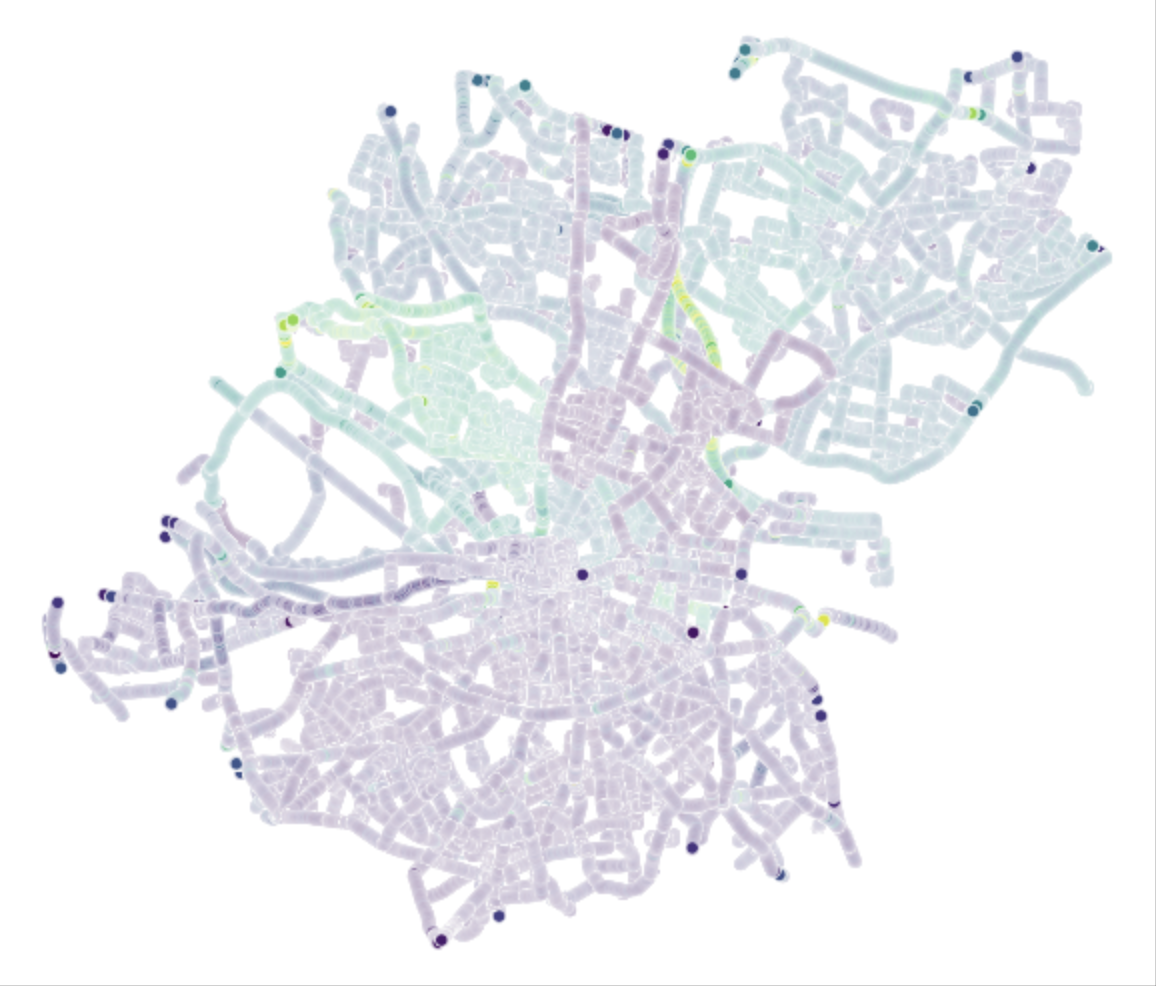
\includegraphics[width=0.65\textwidth, trim=20 20 20 20, clip]{heatmap_dublin_pollution.png}
		
		\vfill
		
		\begin{flushleft}
			\begin{tabular}{@{}ll}
				\textbf{Module:}      & Intro to Machine Learning \\
				\textbf{Programme:}    & MSc in Applied Social Data Science \\
				\textbf{Institution:}  & Trinity College Dublin \\
				\textbf{Authors:}      & Ellen Beattie, Jakob L\"utkemeier, Roudra Sarkar, Rosalie LaCroix \\
				\textbf{Date:}         & April 2, 2026 \\
			\end{tabular}
		\end{flushleft}
		
	\end{titlepage}
	
	% ============================================================
	% 1. OBJECTIVE AND MOTIVATION
	% ============================================================
	\section{Objective and motivation}
	
	This project investigates factors associated with air pollution in Dublin and develops a forecasting model for next-day PM2.5. The project is not solely about predictive accuracy; it asks whether a usable, policy-relevant next-day signal can be extracted from the available data.
	
	We focused on PM2.5 because fine particulate matter is widely recognised as one of the most harmful air pollutants for human health~\cite{ourworldindata}. PM2.5 refers to particulate matter smaller than 2.5 micrometres in diameter~\cite{yang2020}. It has been found to decrease visibility, penetrate the lungs, and harm the respiratory, cardiovascular, cerebrovascular, and nervous systems~\cite{yang2020}. It is also closely related to mortality~\cite{yang2020}.
	
	The practical aim of this work is to inform monitoring, communication, and intervention timing for Dublin City Council (DCC)~\cite{dcc}. DCC should therefore treat the results of this project as a proof of concept for short-term PM2.5 forecasting, one that can guide decisions about where to invest in better data infrastructure and operational tools.
	
	% ============================================================
	% 2. DATA
	% ============================================================
	\section{Data}
	
	Three data sources underpin this project: Google Air View mobile pollution measurements, Met \'Eireann weather records, and SCATS traffic volumes. PM2.5 is the target pollutant, weather captures major naturogenic influences on particulate dispersion, and traffic captures a principal anthropogenic emission source in an urban setting. Meteorological conditions, emissions, and external transport have been found to influence atmospheric particulate matter concentrations~\cite{yang2020}, while in urban areas the main human-generated sources include exhaust emissions, road surface abrasion, brake and tyre wear, and particle resuspension from paved roadways~\cite{karagulian2015}.
	
	\subsection*{Google Air View data}
	
	The core dataset consists of street-view car pollutant measurements recorded at one-second intervals whenever the vehicle was operating over a 15-month period (May 2021--August 2022), containing more than five million timestamped mobile observations linked to GPS coordinates. The data reflect daytime mobile observations taken across Dublin city, not a fixed-station monitoring system. After cleaning and aggregation, the final All-Dublin analytical dataset contained 286 observed Dublin weekdays.
	
	A major strength of the Air View data is its unusually rich spatial detail. It provides high-resolution street-level measurements relevant to exposure patterns across Dublin. Its main weaknesses are that coverage is mobile, uneven, and weekday-only, with daily observation counts varying substantially. Rush-hour data before 9\,am and after 6\,pm, as well as weekend and public holiday observations, are absent. The data are therefore sufficient for a city-wide next-observed-weekday forecasting exercise, but not for a full seven-day, 24-hour ambient forecasting system, and are better suited to a Dublin-wide daily average target than to highly local forecasting.
	
	%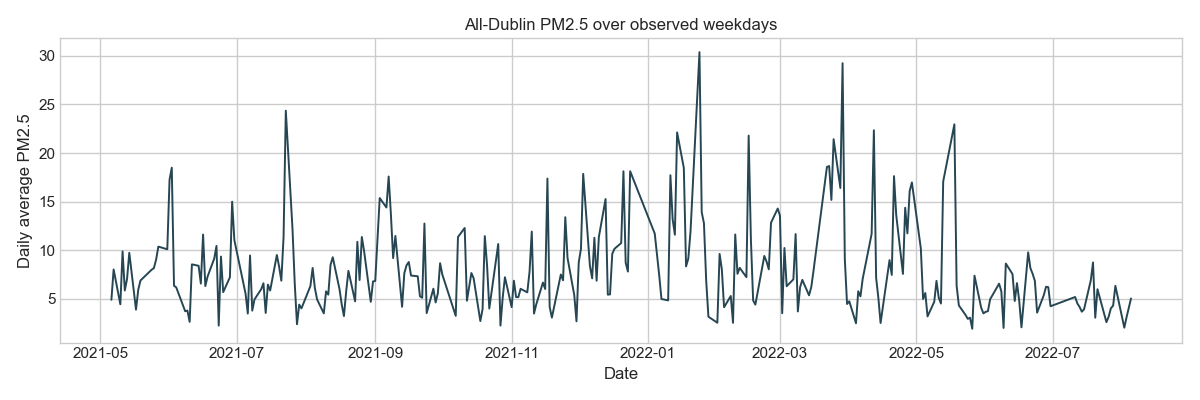
\includegraphics[width=0.95\textwidth]{average_pm25_linechart.png}
	%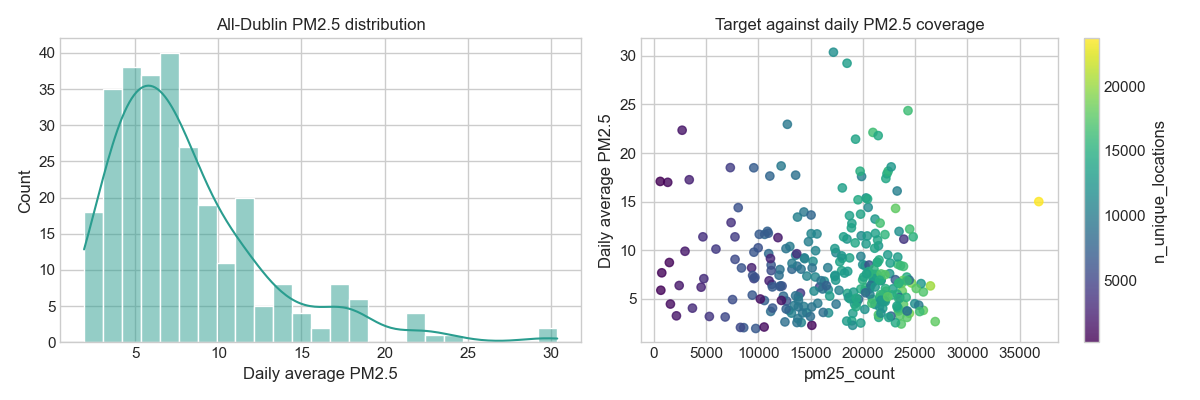
\includegraphics[width=0.95\textwidth]{distribution_PM25.png}
	
	\subsection*{Weather and traffic data}
	
	Weather data were taken from Met \'Eireann's Dublin Airport daily series~\cite{metdata}. These provided several promising candidate predictors, motivated by prior literature and later assessed in our own exploratory scatterplots, including windspeed, temperature, and evaporation-related measures~\cite{yang2020}. Traffic data come from the Sydney Coordinated Adaptive Traffic System (SCATS), which uses sensors at each traffic signal to detect vehicle presence~\cite{scatsdata}. The dataset provides total and average traffic volumes for the preceding hour. These data were initially available at region-day level and were later aligned to the Dublin-wide target through spatial aggregation.
	
	\vspace{2cm}
	
	% ============================================================
	% 3. FACTOR CHOICE
	% ============================================================
	\section{Factor choice}
	
	\subsection*{Data preparation}
	
	During visualisation the data were explored to reveal coverage restrictions, relationships between variables, descriptive statistics, spread, granularity, and missingness. The Air View data showed that weekends were not present and that there were fewer recordings on Mondays and Fridays. For preprocessing, any PM2.5 value above 400 was removed after consultation with a news article indicating that such readings could be reported as anomalies~\cite{breakingnews}. From the weather data only columns potentially correlated with PM2.5 were retained, and from the traffic data only the mean, median, and total daily site volumes were kept.
	
	All data were aggregated by location using averages across Dublin for PM2.5 and traffic measurements; weather was recorded at only one location (Dublin Airport). This was a pragmatic decision to align the observational unit across all three data sources. It makes the modelling problem tractable and defensible given the available weather and traffic data, and it means the results speak to city-wide daily conditions rather than local hotspots. The Air View data were aggregated in two explicit stages: first from timestamp to date, and then from many within-day GPS points to one Dublin-wide daily average PM2.5 target. All datasets were then merged by date, including variables for day of the week, day name, and the averaged pollution, weather, and traffic data.
	
	Weekends are structurally out of scope rather than random missing observations, and even after accounting for that, the dataset still contains some unexpected missing weekdays. Coverage diagnostics suggest the target is reasonably stable, but uneven observation counts remain a real limitation.
	
	\subsection*{Exogenous variable selection}
	
	Predictor selection aimed to keep the final model parsimonious and interpretable. Redundant or overlapping variables were removed to reduce noise and unnecessary complexity, which was especially important given the modest city-day sample size. Correlation matrices between traffic variables and PM2.5 values and between weather variables and PM2.5 values were used to guide selection.
	
	For traffic, Dublin mean traffic values were chosen because the mean had a larger spread of values than the median and total. The final traffic variable used was \texttt{dublin\_mean\_site\_traffic}.
	
	%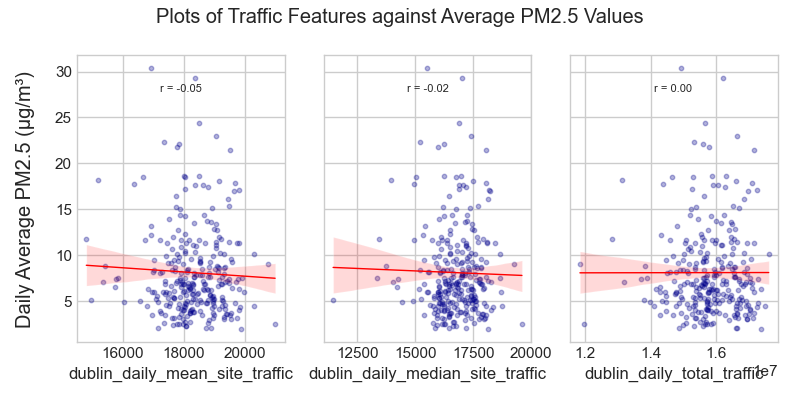
\includegraphics[width=0.95\textwidth]{traffic_features_scatter.png}
	
	For weather, three variables were dropped. Rainfall did not appear to be related to PM2.5 levels in exploratory inspection. Potential evapotranspiration (\texttt{pe}) was highly correlated with evaporation and is conceptually very similar. The highest 10-minute windspeed (\texttt{hm}) was dropped because other, more influential wind measures were available. The final weather variables retained were: \texttt{maxtp} (maximum temperature), \texttt{mintp} (minimum temperature), \texttt{wdsp} (mean wind speed in knots), \texttt{hg} (highest gust in knots), \texttt{sun} (sunshine duration in hours), \texttt{g\_rad} (global radiation in J/cm\textsuperscript{2}), and \texttt{evap} (evaporation in mm).
	
	%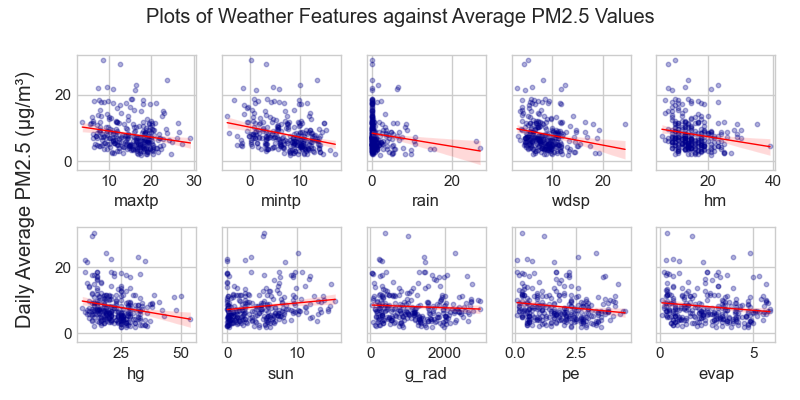
\includegraphics[width=1.1\textwidth]{weather_features_scatter.png}
	%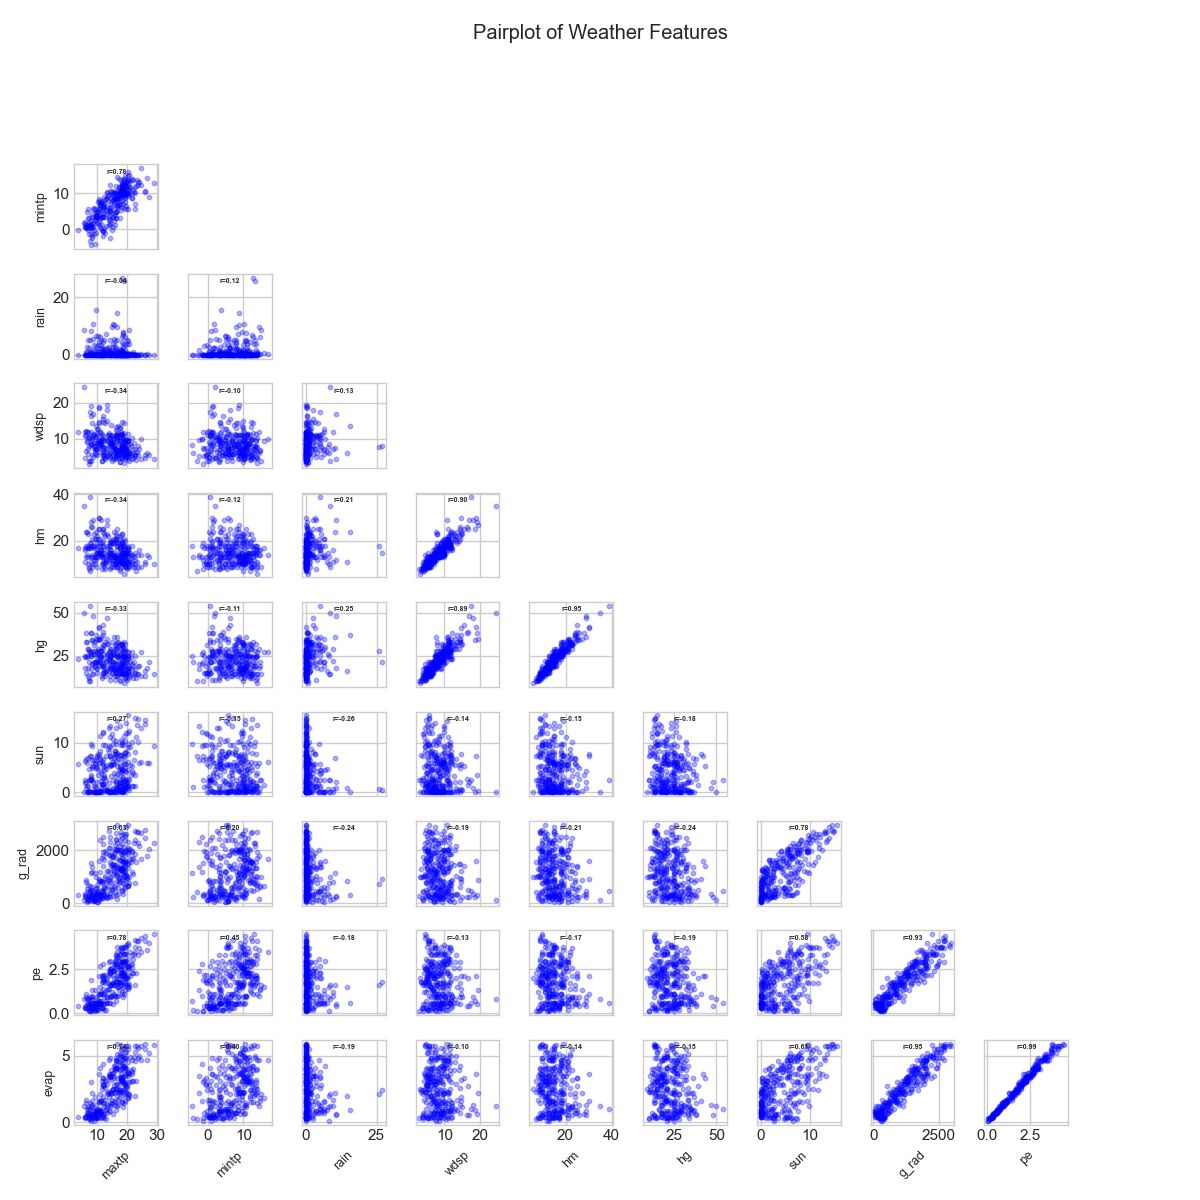
\includegraphics[width=1.2\textwidth]{weather_features_pairplot.png}
	
	\subsection*{Temporal feature selection}
	
	No strong seasonality or long-run trend was noted over the study period. Daily averages appear to change slightly by weekday, indicating that \texttt{day\_of\_week} is beneficial to include in the model. Temporal diagnostics supported a short lag structure, with \texttt{lag\_1} as the strongest single predictor and lags 2 and 3 showing weaker but still useful additional signal. The final temporal features were \texttt{day\_of\_week}, \texttt{lag\_1}, \texttt{lag\_2}, and \texttt{lag\_3}.
	
	\vspace{2cm}
	
	%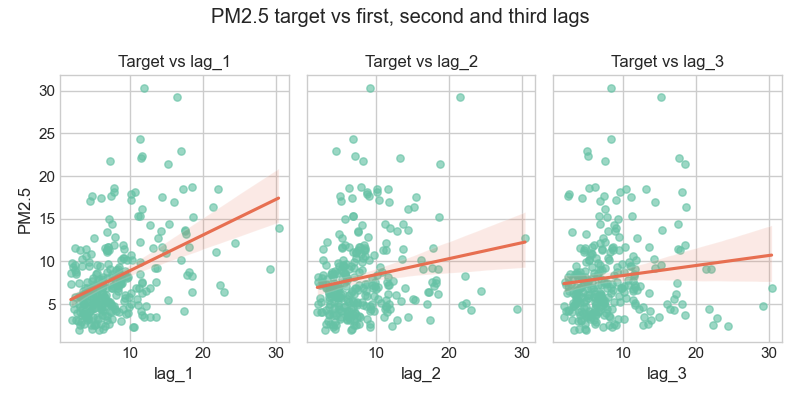
\includegraphics[width=0.5\textwidth]{target_vs_lag_scatter.png}
	%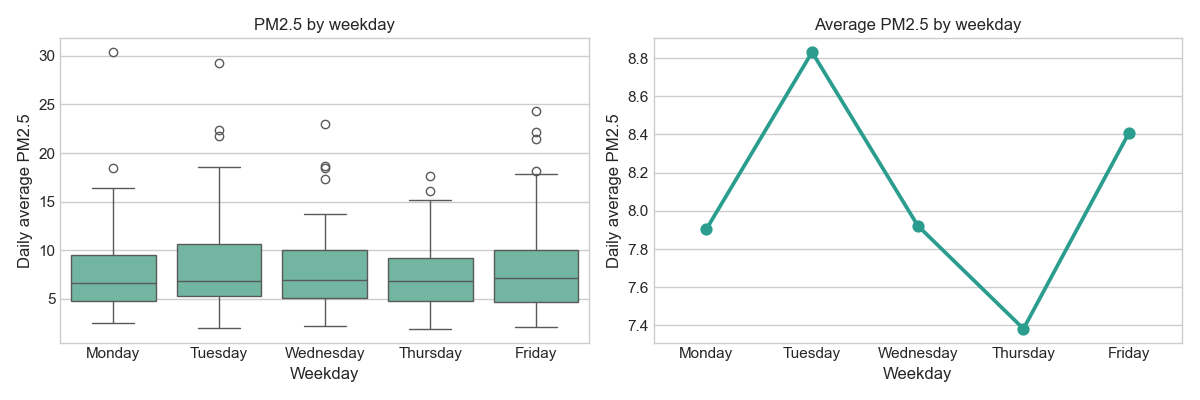
\includegraphics[width=0.95\textwidth]{weekday_avgPM25.png}
	
	% ============================================================
	% 4. METHOD
	% ============================================================
	\section{Method}
	
	\subsection*{Train/test split}
	
	A single shared chronological train--test split was created on the observed rows. The split is designed to preserve the forward-looking forecasting setting, so all models are evaluated on a genuinely held-out future period. This avoids leakage from future observations into training. All subsequent models draw from this split and then apply any model-specific preprocessing afterwards, ensuring accurate and consistent comparisons between models.
	
	\subsection*{Baseline model}
	
	The most basic model was used to obtain evaluation metrics against which more complex models could be compared. This baseline predicts each observed test-day PM2.5 value using the previous observed PM2.5 value; the first test prediction therefore uses the last observed training value.
	
	\subsection*{Linear Regression}
	
	This model used the past three days of data from all variables to create a weighted, linear combination of these predictors. It is simple and easy to interpret, showing how PM2.5 values change as a function of the selected predictors.
	
	\subsection*{Direct One-Step-Ahead Ridge ARX}
	This is a suitable full model for the project because the task is one-step-ahead prediction, the sample is relatively small, and several retained weather variables remain correlated. Ridge regularisation shrinks unstable coefficients without sacrificing interpretability, making it a sensible ARX specification for a compact city-day dataset. Cross-validation on the training data was used to select the optimal value of the regularisation parameter \(\lambda\). A key principle is that the model uses only information that would actually be available at forecast time: weather and traffic therefore enter in lagged form rather than as tomorrow's realised values. This makes the forecasting exercise more realistic but also more demanding.
	
	\subsection*{Random Forest}
	This model provides a contrasting non-linear benchmark to the linear and ridge regressions, helping assess whether a more flexible forecasting approach adds value beyond the simpler specifications.
	
	% ============================================================
	% 5. RESULTS
	% ============================================================
	\section{Results}
	
	The models were compared using root mean squared error (RMSE) on the held-out test set. The results are summarised below:
	
	\begin{table}[H]
		\centering
		\caption{RMSE comparison across models.}
		\label{tab:rmse}
		\begin{tabular}{@{}lc@{}}
			\toprule
			\textbf{Model} & \textbf{RMSE} \\
			\midrule
			Baseline (persistence) & 3.86 \\
			Linear regression      & 3.94 \\
			Direct one-step-ahead Ridge ARX & 3.72 \\
			Random forest          & 4.62 \\
			\bottomrule
		\end{tabular}
	\end{table}
	
	The direct one-step-ahead Ridge ARX model delivered the best held-out performance. However, the improvement over the simple persistence baseline is modest, which suggests that most short-term predictability comes from recent PM2.5 history. Weather and traffic add incremental signal, but they do not transform forecast accuracy.
	
	This indicates that the strongest short-term predictive signal is temporal persistence. The random forest did not outperform the more interpretable linear-style models, suggesting that forecast gains came more from careful feature design than from additional model complexity.
	
	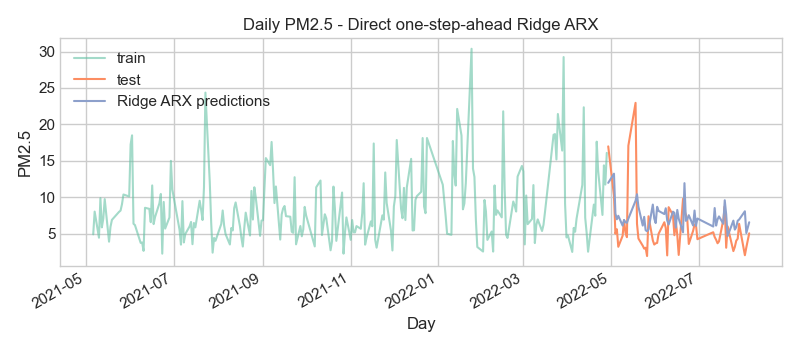
\includegraphics[width=0.95\textwidth]{ridgeARX_pred.png}
	
	% ============================================================
	% 6. DISCUSSION AND RECOMMENDATION
	% ============================================================
	\section{Discussion and recommendation}
	
	\subsection*{Main findings}
	
	The project achieved modest but meaningful next-day PM2.5 predictive performance using the data, features, processing, and model tuning implemented here. The strongest and most defensible predictive signal is temporal persistence, especially yesterday's PM2.5. The project therefore supports a light-touch next-day decision-support tool; it does not yet support a highly accurate standalone operational forecasting system.
	
	\subsection*{Limitations}
	
	The weather data may not be fully representative of conditions across Dublin because they come from a single fixed location at Dublin Airport. With weather data recorded closer to, or within, the city centre, PM2.5 predictions for the city would likely be more accurate. Because the observational regime is weekday-only, weekend coverage would improve continuity and generalisability. Better location indicators and more spatially balanced monitoring would also allow the data to be disaggregated for location-specific forecasts.
	
	The All-Dublin aggregation is sensible for the main model, but it necessarily masks neighbourhood-level variation. The limited gains from weather and traffic should not be read as evidence that those factors are unimportant; their predictive value is constrained by using only information available at forecast time (\(t-1\)).
	
	\subsection*{Recommendations}
	
	DCC should treat this as a proof of concept for short-term PM2.5 forecasting and as a light-touch decision-support tool rather than a standalone operational forecast. The most valuable next improvements are likely to come from better temporal continuity, more spatially balanced monitoring, more local weather inputs, and forecast weather and forward-looking traffic inputs. Better data design is likely to yield more policy value than simply moving to more complex algorithms.
	
	\vspace{5cm}
	
	% ============================================================
	% REFERENCES
	% ============================================================
	\begin{thebibliography}{9}
		
		\bibitem{yang2020}
		Yang, H., Peng, Q., Zhou, J. \emph{et al.} The unidirectional causality influence of factors on PM2.5 in Shenyang city of China. \emph{Sci Rep} \textbf{10}, 8403 (2020). \url{https://doi.org/10.1038/s41598-020-65391-5}
		
		\bibitem{karagulian2015}
		Karagulian, F., Belis, C.\,A., Dora, C.\,F.\,C. \emph{et al.} Contributions to cities' ambient particulate matter (PM): A systematic review of local source contributions at global level. \emph{Atmospheric Environment} (2015). \url{https://www.sciencedirect.com/science/article/pii/S0169809512003237}
		
		\bibitem{breakingnews}
		Breaking News, ``Dublin's air pollution hits highest levels since the 1980s.'' \url{https://www.breakingnews.ie/ireland/dublins-air-pollution-hits-highest-levels-since-the-1980s-1044551.html}
		
		\bibitem{metdata}
		Met \'Eireann, Dublin Airport daily data. \url{https://data.gov.ie/en_GB/dataset/dashboard/dublin-airport-daily-data}
		
		\bibitem{scatsdata}
		Smart Dublin, Traffic volumes from SCATS traffic management system (2021--2022). \url{https://data.gov.ie/dataset/traffic-volumes-from-scats-traffic-management-system-2021}
		
		\bibitem{ourworldindata}
		Our World in Data, Air pollution sources. \url{https://ourworldindata.org/air-pollution-sources}
		
		\bibitem{dcc}
		Dublin City Council, Controlling air pollution. \url{https://www.dublincity.ie/environment-and-climate-action/controlling-air-pollution}
		
	\end{thebibliography}
	
\end{document}